% ======================================================================
\documentclass[12pt,a4paper,twoside,openright]{book}

%───────── Plantilla, portadas y contraportada ─────────────────────────
\usepackage{template/sty_files/template-TFGspanish-uma}

\usepackage{template/sty_files/cotutor_cover-blueuma}
\usepackage{template/sty_files/cotutor_cover-whiteuma}

\usepackage{template/sty_files/backcover-umaes}

%───────── Paquetes auxiliares ─────────────────────────────────────────
\usepackage{blindtext}
\usepackage{mwe}               
\usepackage{csquotes}
\usepackage{float}
\usepackage{enumitem}
\usepackage[
  backend=bibtex,
  style=numeric,
  sorting=nyt
]{biblatex}
\usepackage{setspace}
\usepackage{tabularx}
\onehalfspacing
\addbibresource{sections/Referencias/references.bib}
\setlength{\parskip}{0.6em}
\setlength{\parindent}{0pt}
\setlist[enumerate]{nosep}
\raggedbottom

%======================================================================
\begin{document}

%────────────────────── Blue front cover ───────────────────────────────
\MakeBlueUMACover{
  degree     = {Grado en Ingeniería Informática},
  mencion    = {Mención en Computación},
  titleES    = {Análisis del rendimiento y consumo de modelos de IA para detección de intrusiones},
  titleEN    = {Performance and consumption analysis of AI models for intrusion detection},
  author     = {Plácido Velasco Muñoz},
  tutor      = {Dr. Rodrigo Román Castro},
  cotutor    = {Dr. Francisco José Jaime Rodríguez},
  dept       = {Departamento de Lenguajes y Ciencias de la Computación},
  cityDate   = {Málaga, \today},
  logoLeft   = {template/logos/NEG-uma-logo.png},
  logoRight  = {template/logos/NEG-etsi-logo.png}
}


%────────────────────── White front cover ──────────────────────────────
\MakeWhiteUMACover{
  degree     = {Grado en Ingeniería Informática},
  mencion    = {Mención en Computación},
  titleES    = {Análisis del rendimiento y consumo de modelos de IA para detección de intrusiones},
  titleEN    = {Performance and consumption analysis of AI models for intrusion detection},
  author     = {Plácido Velasco Muñoz},
  tutor      = {Dr. Rodrigo Román Castro},
  cotutor    = {Dr. Francisco José Jaime Rodríguez},
  dept       = {Departamento de Lenguajes y Ciencias de la Computación},
  cityDate   = {Málaga, \today},
  defenseDate = {septiembre de 2025},
  logoLeft    = {template/logos/POS-uma-logo.png},
  logoRight   = {template/logos/POS-etsi-logo.png}
}
\frontmatter

%────────────────────── Resumen / Abstract ─────────────────────────────
\renewcommand{\abstractname}{Resumen}

\begin{abstract}

En el ámbito de la ciberseguridad, los sistemas de detección de intrusiones (IDS) desempeñan un papel fundamental para la
identificación temprana de ataques y actividades maliciosas en redes informáticas. En los últimos años, el uso de técnicas de
inteligencia artificial (IA) y aprendizaje automático (Machine Learning) ha permitido mejorar significativamente la precisión
y la capacidad de adaptación de estos sistemas frente a amenazas cada vez más complejas y dinámicas. \\
    
Sin embargo, gran parte de la investigación existente se ha centrado principalmente en mejorar la tasa de detección o reducir los
falsos positivos, sin considerar en profundidad el impacto computacional y energético que conllevan estos modelos. En entornos
donde el procesamiento debe realizarse en tiempo real (como redes corporativas, sistemas embebidos o infraestructuras
críticas) el consumo de recursos (CPU, memoria, GPU) y la latencia de inferencia se convierten en factores determinantes para
la viabilidad de la solución. \\

El proyecto se enfoca en el análisis, evaluación, selección de hiperparámetros y configuración de modelos de IA para comparar el rendimiento y eficiencia computacional de los distintos modelos aplicados a la detección de intrusiones.

Además, se hace un análisis posterior para ver como los mejores modelos reaccionan ante diferentes técnicas de evasión.



\medskip
\noindent\textbf{Palabras clave:} 
sistemas de detección de intrusiones (IDS), ataques adversarios, Internet de las Cosas (IoT), eficiencia computacional, frontera de pareto 
\end{abstract}

\renewcommand{\abstractname}{Abstract}
\begin{abstract}

In the field of cybersecurity, intrusion detection systems (IDS) play a vital role in the
early identification of attacks and malicious activity on computer networks. In recent years, the use of
artificial intelligence (AI) and machine learning techniques has significantly improved the accuracy
and adaptability of these systems in the face of increasingly complex and dynamic threats. \\
    
However, much of the existing research has focused primarily on improving the detection rate or reducing
false positives, without thoroughly considering the computational and energy impact of these models. In environments
where processing must be carried out in real time (such as corporate networks, embedded systems or critical
infrastructure), resource consumption (CPU, memory, GPU) and inference latency become determining factors for
the viability of the solution. \\

The project focuses on the analysis, evaluation, hyperparameter selection and configuration of AI models to compare the performance and computational efficiency of the various models applied to intrusion detection.

Furthermore, a subsequent analysis is carried out to examine how the best models react to different evasion techniques.

\medskip
\noindent\textbf{Keywords:} 
intrusion detection systems (IDS), cyberattacks, the Internet of Things (IoT), computational efficiency, pareto frontier
\end{abstract}

%──────────────── Agradecimientos ──────────────────────────────────────
% Sección opcional, si no se quiere usar, borrar el entorno umaacknowledgments

% Descomentar si los vas a escribir en inglés
% \SetAcknowledgmentsName{Acknowledgments} 
\begin{umaacknowledgments}

\end{umaacknowledgments}

%────────────────────── Índice y listas ────────────────────────────────
\clearpage
\tableofcontents
\clearpage
\listoffigures
\clearpage
\listoftables
\clearpage

%────────────────────── Nomenclatura ───────────────────────────────────
\nomenclature{}{}
\printnomenclature
\clearpage

\mainmatter
%────────────────────── Cuerpo ─────────────────────────────────────────
% https://en.wikipedia.org/wiki/Standing_on_the_shoulders_of_giants 

\chapter{Investigación Previa}
\subsection{Machine Learning}

El \textit{Machine Learning} (aprendizaje automático) es una rama de la inteligencia artificial que permite a los sistemas aprender y mejorar automáticamente a partir de la experiencia, sin ser programados explícitamente para cada tarea. Utiliza algoritmos que identifican patrones en grandes volúmenes de datos y toman decisiones o realizan predicciones basadas en esos patrones.

En el contexto de los Sistemas de Detección de Intrusos (IDS), el \textit{Machine Learning} se emplea para analizar el tráfico de red y detectar comportamientos anómalos o maliciosos de manera más eficiente y precisa que los métodos tradicionales basados en firmas. Además, la relación con la \textit{Green AI} surge porque el uso de técnicas de aprendizaje automático más eficientes puede reducir el consumo energético, promoviendo soluciones más sostenibles.

\subsubsection{Random Forest (RF)}

\textbf{Random Forest} es un algoritmo de aprendizaje supervisado basado en un ensamblado de árboles de decisión entrenados de forma independiente. El modelo construye múltiples árboles utilizando distintas muestras del conjunto de entrenamiento obtenidas mediante \textit{bootstrap sampling}, así como subconjuntos aleatorios de características en cada división. La predicción final se obtiene combinando las salidas de todos los árboles, habitualmente mediante votación mayoritaria en tareas de clasificación.

A diferencia de los métodos de \textit{boosting}, como XGBoost, los árboles que componen un Random Forest no se entrenan de manera secuencial ni dependen unos de otros. Cada árbol aprende de forma autónoma a partir de una vista ligeramente distinta de los datos, lo que permite reducir la varianza del modelo y mejorar su robustez frente al ruido y al sobreajuste. Esta independencia entre árboles hace que Random Forest sea especialmente estable y fiable como modelo base en problemas de detección de intrusiones.

Desde el punto de vista de la inferencia, Random Forest presenta una latencia muy reducida, ya que la predicción consiste únicamente en recorrer un número limitado de árboles poco profundos y agregar sus decisiones. Además, al no requerir cálculos iterativos complejos ni funciones de activación costosas, su consumo computacional durante la fase de operación es bajo, lo que lo convierte en una opción adecuada para despliegues en entornos con recursos limitados.

En el contexto de \textit{Green AI}, Random Forest destaca por ofrecer un excelente equilibrio entre rendimiento y eficiencia energética. Aunque el entrenamiento puede ser más costoso que el de un único árbol de decisión, este proceso se realiza de forma puntual y fuera de línea. En contraste, la fase de inferencia es altamente eficiente, lo que resulta especialmente relevante en sistemas de detección de intrusiones que deben operar de forma continua en tiempo real.

\begin{table}[H]
    \centering
    \caption{Principales hiperparámetros de Random Forest y su significado.}
    \label{tab:rf_hyperparams}
    \begin{tabular}{ll}
        \toprule
        \textbf{Hiperparámetro} & \textbf{Significado} \\
        \midrule
        \texttt{n\_estimators} & Número de árboles en el bosque \\
        \texttt{max\_depth} & Profundidad máxima de cada árbol \\
        \texttt{min\_samples\_split} & Mínimo de muestras para dividir un nodo \\
        \texttt{min\_samples\_leaf} & Mínimo de muestras en una hoja \\
        \texttt{max\_features} & Número de características consideradas en cada división \\
        \texttt{bootstrap} & Si se usan muestras con reemplazo para entrenar cada árbol \\
        \texttt{criterion} & Función para medir la calidad de una división (por ejemplo, \textit{gini} o \textit{entropy}) \\
        \bottomrule
    \end{tabular}
\end{table}

\begin{figure}[H]
    \centering
    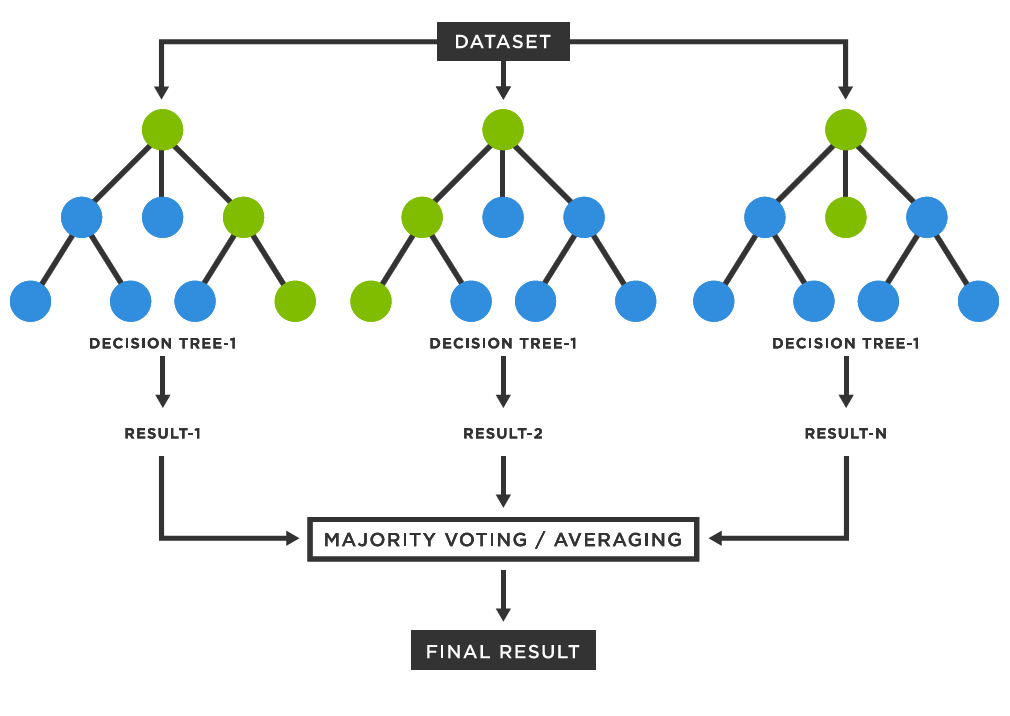
\includegraphics[width=0.7\textwidth]{images/random_forest.png}
    \caption{Esquema representativo del funcionamiento de Random Forest.}
    \label{fig:randomforest}
\end{figure}

\subsubsection{Extreme Gradient Boosting (XGBoost)}

\textbf{XGBoost} (\textit{Extreme Gradient Boosting}) es un algoritmo de aprendizaje supervisado basado en árboles de decisión que implementa de forma altamente optimizada el principio de \textit{gradient boosting}. A diferencia de otros métodos basados en ensamblados de árboles, XGBoost construye el modelo de manera secuencial, añadiendo nuevos árboles que se centran en corregir los errores cometidos por los árboles previamente entrenados. Este proceso se basa en la optimización iterativa de una función objetivo que combina el error de clasificación con términos explícitos de regularización, lo que permite controlar la complejidad del modelo y reducir el sobreajuste.

En cada iteración, XGBoost utiliza información de primer y segundo orden del gradiente de la función de pérdida para determinar la estructura óptima de los árboles, lo que le permite capturar relaciones no lineales complejas e interacciones entre características de forma eficiente. Estas propiedades lo convierten en una opción especialmente adecuada para la detección de intrusiones en conjuntos de datos tabulares, donde los patrones maliciosos suelen manifestarse a través de combinaciones no triviales de múltiples variables.

En XGBoost, la predicción final del modelo no corresponde a la salida de un único árbol de decisión, sino que se obtiene como la combinación aditiva de las salidas de todos los árboles entrenados. Cada árbol aporta una contribución parcial a la predicción, y el resultado final se calcula sumando dichas contribuciones.
El proceso de entrenamiento es secuencial: cada nuevo árbol se entrena para corregir los errores residuales cometidos por el conjunto de árboles previamente construidos. Como consecuencia, el último árbol no contiene una decisión completa por sí mismo, sino que únicamente modela aquellos patrones que aún no han sido correctamente capturados por los árboles anteriores, actuando como un ajuste fino del modelo global.
De este modo, XGBoost se centra en la reducción del sesgo, lo que suele traducirse en un mayor rendimiento predictivo cuando se dispone de un número limitado de características relevantes.

En el contexto de este trabajo, la elección de XGBoost resulta especialmente adecuada al considerar criterios de eficiencia computacional y sostenibilidad, en línea con los principios de \textit{Green AI}. Aunque el proceso de entrenamiento de XGBoost puede ser más costoso que el de otros modelos clásicos, este se realiza de forma puntual y fuera de línea. En cambio, la fase de inferencia presenta una latencia muy reducida, ya que únicamente requiere recorrer un número limitado de árboles poco profundos, lo que lo hace compatible con despliegues en entornos \textit{edge} e IoT. Por tanto, XGBoost ofrece un equilibrio muy favorable entre rendimiento y coste computacional, permitiendo alcanzar altas tasas de detección sin incurrir en un consumo energético elevado durante la operación del sistema IDS.

\begin{table}[H]
    \centering
    \caption{Principales hiperparámetros de XGBoost y su significado.}
    \label{tab:xgboost_hyperparams}
    \begin{tabular}{ll}
        \toprule
        \textbf{Hiperparámetro} & \textbf{Significado} \\
        \midrule
        \texttt{n\_estimators} & Número de árboles a construir \\
        \texttt{max\_depth} & Profundidad máxima de cada árbol \\
        \texttt{learning\_rate} & Tasa de aprendizaje (contribución de cada árbol) \\
        \texttt{subsample} & Proporción de muestras usadas en cada iteración \\
        \texttt{colsample\_bytree} & Proporción de características usadas por árbol \\
        \texttt{gamma} & Mínima reducción de pérdida para dividir un nodo \\
        \texttt{reg\_alpha} & Término de regularización L1 \\
        \texttt{reg\_lambda} & Término de regularización L2 \\
        \texttt{objective} & Función objetivo a optimizar (por ejemplo, \textit{binary:logistic}) \\
        \bottomrule
    \end{tabular}
\end{table}

\begin{figure}[H]
    \centering
    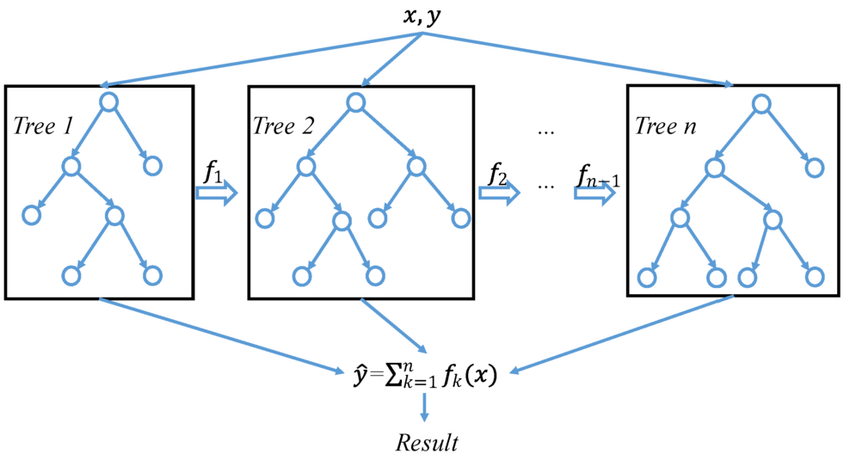
\includegraphics[width=0.7\textwidth]{images/xg_boost.png}
    \caption{Esquema representativo del funcionamiento de XGBoost.}
    \label{fig:xgboost}
\end{figure}

\subsubsection{Support Vector Machine (SVM)}

\textbf{Support Vector Machines} (SVM) es un algoritmo de aprendizaje supervisado cuyo objetivo principal es encontrar una frontera de decisión que separe de forma óptima las distintas clases en el espacio de características. En su formulación básica, SVM busca el hiperplano que maximiza el margen entre las muestras de distintas clases, utilizando únicamente un subconjunto de los datos denominado \textit{vectores soporte}. Esta propiedad permite construir modelos robustos frente al ruido y con buena capacidad de generalización.

Una de las principales fortalezas de las SVM es el uso de \textit{kernels}, que permiten proyectar los datos originales a espacios de mayor dimensionalidad sin realizar explícitamente dicha transformación. Gracias a este mecanismo, SVM puede modelar fronteras de decisión no lineales incluso cuando los datos no son separables linealmente en el espacio original. Entre los kernels más utilizados se encuentran:

\begin{itemize}
    \item \textbf{Kernel lineal}: Define una frontera de decisión lineal en el espacio de características original. Es el kernel más simple y el más eficiente desde el punto de vista computacional, lo que lo hace especialmente adecuado para datasets de gran tamaño y para escenarios donde se prioriza la eficiencia.
    
    \item \textbf{Kernel polinómico}: Permite modelar relaciones no lineales mediante funciones polinómicas de distinto grado. Aunque puede capturar interacciones más complejas entre las características, su coste computacional aumenta rápidamente con el grado del polinomio y el tamaño del dataset.
    
    \item \textbf{Kernel radial (RBF)}: Proyecta los datos a un espacio de dimensión infinita, permitiendo separar patrones altamente no lineales. Si bien suele ofrecer un alto rendimiento predictivo, su entrenamiento e inferencia son significativamente más costosos, especialmente en conjuntos de datos de gran tamaño.
\end{itemize}

En el contexto de este trabajo, el uso de SVM se plantea principalmente mediante un \textbf{kernel lineal}, ya que ofrece un compromiso adecuado entre rendimiento y eficiencia computacional. Los kernels no lineales, como el RBF, resultan poco escalables para los volúmenes de datos considerados y presentan un coste energético elevado, lo que los hace menos compatibles con los principios de \textit{Green AI}.

\begin{table}[H]
    \centering
    \caption{Principales hiperparámetros de SVM y su significado.}
    \label{tab:svm_hyperparams}
    \begin{tabular}{ll}
        \toprule
        \textbf{Hiperparámetro} & \textbf{Significado} \\
        \midrule
        \texttt{C} & Parámetro de regularización que controla el equilibrio entre margen y error de clasificación \\
        \texttt{kernel} & Tipo de función kernel utilizada (por ejemplo, \textit{linear}, \textit{poly}, \textit{rbf}) \\
        \texttt{degree} & Grado del polinomio (solo para kernel polinómico) \\
        \texttt{gamma} & Coeficiente para kernels \textit{rbf}, \textit{poly} y \textit{sigmoid} \\
        \texttt{coef0} & Término independiente en kernels \textit{poly} y \textit{sigmoid} \\
        \bottomrule
    \end{tabular}
\end{table}

\begin{figure}[H]
    \centering
    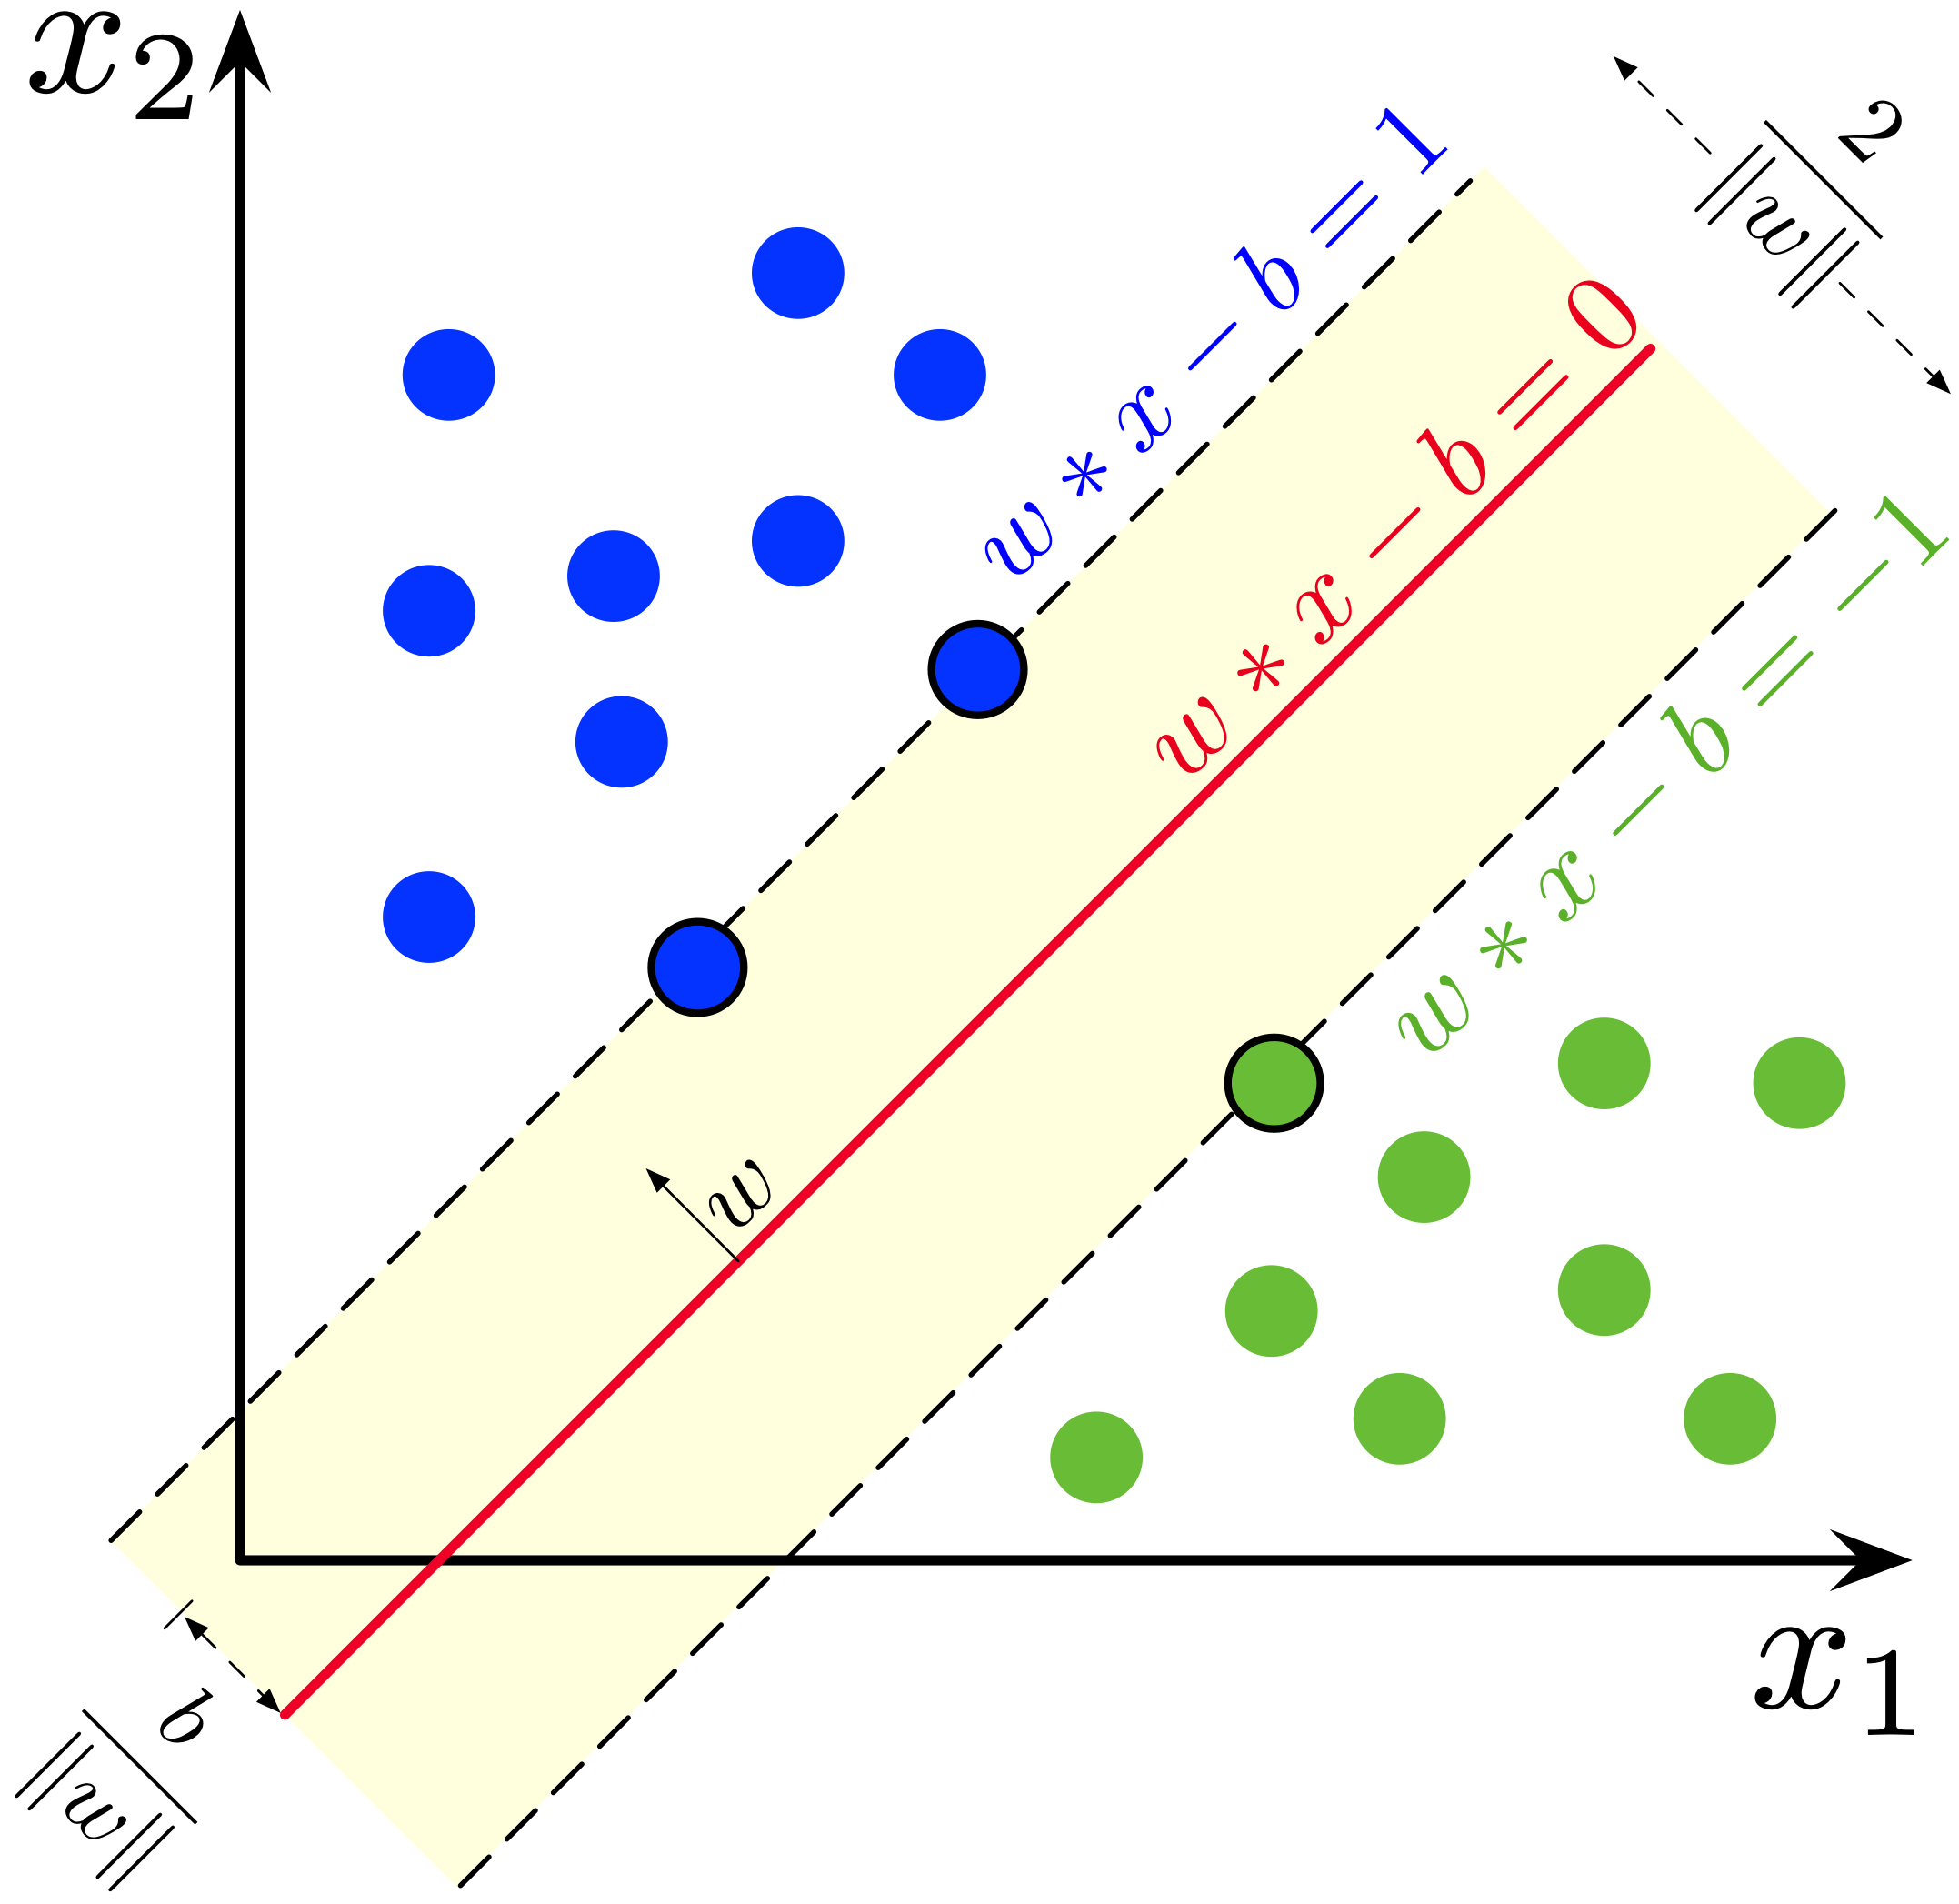
\includegraphics[width=0.5\textwidth]{images/SVM_margin.png}
    \caption{Ejemplo de separación óptima de clases mediante SVM y margen máximo.}
    \label{fig:svm_margin}
\end{figure}

\subsection{Deep Learning}

El \textit{Deep Learning} (aprendizaje profundo) es una subárea del aprendizaje automático que se basa en redes neuronales artificiales con múltiples capas (redes neuronales profundas). Estas redes son capaces de aprender representaciones jerárquicas de los datos, lo que les permite capturar patrones complejos y realizar tareas como clasificación, reconocimiento de imágenes y procesamiento del lenguaje natural.

En el ámbito de los IDS, el \textit{Deep Learning} se utiliza para mejorar la detección de intrusiones mediante la capacidad de aprender características complejas del tráfico de red. Sin embargo, es importante considerar que los modelos de aprendizaje profundo suelen requerir una gran cantidad de datos y recursos computacionales, lo que puede aumentar el consumo energético. Por lo tanto, es crucial buscar enfoques que optimicen el rendimiento sin comprometer la eficiencia energética, alineándose con los principios de la \textit{Green AI}.

\subsubsection{Multilayer Perceptron (MLP)}

El \textbf{Multi-Layer Perceptron} (MLP) es una red neuronal artificial de tipo \textit{feed-forward} compuesta por una capa de entrada, una o varias capas ocultas y una capa de salida. Cada capa está formada por neuronas completamente conectadas, donde cada neurona realiza una combinación lineal de sus entradas seguida de una función de activación no lineal. Este tipo de arquitectura permite aproximar funciones no lineales complejas y es uno de los modelos más utilizados como punto de partida en problemas de aprendizaje profundo.

En el contexto de datasets tabulares, como los empleados en este trabajo, el MLP actúa como un modelo de referencia dentro del aprendizaje profundo, permitiendo evaluar si la introducción de capas no lineales aporta mejoras significativas frente a modelos clásicos como Random Forest o XGBoost. A diferencia de estos últimos, el rendimiento de un MLP depende en gran medida del diseño de la arquitectura y de la correcta selección de hiperparámetros.

Desde el punto de vista computacional, su coste está directamente relacionado con el número de capas ocultas y el número de neuronas por capa. Arquitecturas profundas o excesivamente anchas incrementan de forma notable el tiempo de entrenamiento y el consumo de memoria, sin garantizar necesariamente mejoras en el rendimiento para datos tabulares. Por este motivo, en este trabajo se utilizan arquitecturas MLP compactas, con un número reducido de capas y neuronas, priorizando un equilibrio adecuado entre capacidad de modelado y eficiencia computacional.

En términos de \textit{Green AI}, el MLP representa una alternativa intermedia entre los modelos de aprendizaje automático clásico y redes neuronales más complejas como LSTM o CNN. Aunque su entrenamiento es más costoso que el de modelos basados en árboles, la fase de inferencia sigue siendo relativamente eficiente cuando se emplean arquitecturas ligeras, lo que permite analizar el compromiso entre rendimiento y coste computacional en escenarios de detección de intrusiones.

\begin{table}[H]
    \centering
    \caption{Principales hiperparámetros de MLP y su significado.}
    \label{tab:mlp_hyperparams}
    \begin{tabular}{ll}
        \toprule
        \textbf{Hiperparámetro} & \textbf{Significado} \\
        \midrule
        \texttt{hidden\_layer\_sizes} & Número y tamaño de las capas ocultas \\
        \texttt{activation} & Función de activación utilizada en las neuronas (por ejemplo, \textit{relu}, \textit{tanh}) \\
        \texttt{solver} & Algoritmo de optimización para el entrenamiento (por ejemplo, \textit{adam}, \textit{sgd}) \\
        \texttt{alpha} & Parámetro de regularización L2 \\
        \texttt{learning\_rate\_init} & Tasa de aprendizaje inicial \\
        \texttt{batch\_size} & Tamaño del lote de muestras para cada actualización de los pesos \\
        \texttt{max\_iter} & Número máximo de iteraciones de entrenamiento \\
        \texttt{early\_stopping} & Si se detiene el entrenamiento anticipadamente al no mejorar el rendimiento \\
        \bottomrule
    \end{tabular}
\end{table}

\begin{figure}[H]
    \centering
    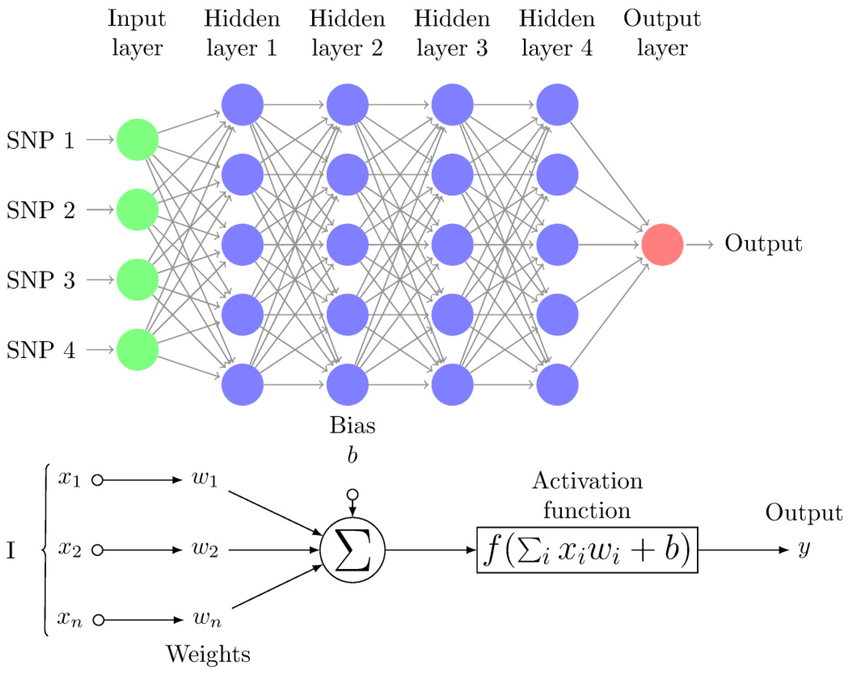
\includegraphics[width=0.7\textwidth]{images/mlp.png}
    \caption{Proceso de retropropagación en una red neuronal MLP.}
    \label{fig:mlp_backpropagation}
\end{figure}

\subsubsection{Long Short-Term Memory (LSTM)}

Las redes \textbf{Long Short-Term Memory} (LSTM) son un tipo de red neuronal recurrente diseñada para modelar dependencias temporales en secuencias de datos. A diferencia de las redes neuronales recurrentes tradicionales, las LSTM incorporan un conjunto de compuertas internas (entrada, olvido y salida) que regulan el flujo de información a lo largo del tiempo, permitiendo conservar o descartar información relevante durante secuencias largas y mitigando el problema del desvanecimiento del gradiente.

En el ámbito de la detección de intrusiones, las LSTM resultan especialmente interesantes cuando el comportamiento malicioso no se manifiesta en observaciones aisladas, sino en patrones temporales que evolucionan a lo largo del tiempo. Aunque los datasets empleados en este trabajo se describen mediante características agregadas a nivel de flujo, el uso de LSTM permite analizar si la introducción de mecanismos de memoria aporta ventajas frente a modelos puramente estáticos, capturando posibles dependencias internas entre características o secuencias de flujos consecutivos.

Desde el punto de vista computacional, las LSTM presentan un coste superior al de modelos \textit{feed-forward} como el MLP, ya que cada unidad recurrente realiza múltiples operaciones internas en cada paso temporal. El número de unidades LSTM y la longitud de las secuencias influyen directamente en el tiempo de entrenamiento y en el consumo de memoria. Por este motivo, en este trabajo se emplean arquitecturas LSTM ligeras, con un número reducido de unidades, evitando configuraciones profundas que resultarían inviables para escenarios con recursos limitados.

En términos de \textit{Green AI}, las LSTM representan un compromiso entre capacidad de modelado y eficiencia. Si bien su entrenamiento e inferencia son más costosos que los de modelos clásicos y MLP sencillos, el uso de configuraciones compactas permite evaluar de forma controlada el impacto de la modelización temporal en el rendimiento del sistema IDS. De este modo, las LSTM se incluyen como un modelo de referencia para analizar el beneficio potencial de incorporar memoria temporal frente al incremento del coste computacional asociado.

\begin{table}[H]
    \centering
    \caption{Principales hiperparámetros de LSTM y su significado.}
    \label{tab:lstm_hyperparams}
    \begin{tabular}{ll}
        \toprule
        \textbf{Hiperparámetro} & \textbf{Significado} \\
        \midrule
        \texttt{units} & Número de unidades LSTM en la capa recurrente \\
        \texttt{return\_sequences} & Si la capa devuelve la secuencia completa o solo el último estado \\
        \texttt{dropout} & Tasa de abandono para regularización durante el entrenamiento \\
        \texttt{recurrent\_dropout} & Tasa de abandono aplicada a las conexiones recurrentes \\
        \texttt{activation} & Función de activación utilizada en las unidades LSTM (por ejemplo, \textit{tanh}) \\
        \texttt{recurrent\_activation} & Función de activación para las compuertas internas (por ejemplo, \textit{sigmoid}) \\
        \texttt{learning\_rate\_init} & Tasa de aprendizaje inicial para el optimizador \\
        \texttt{batch\_size} & Tamaño del lote de muestras para cada actualización de los pesos \\
        \texttt{max\_iter} & Número máximo de iteraciones de entrenamiento \\
        \bottomrule
    \end{tabular}
\end{table}

\begin{figure}[H]
    \centering
    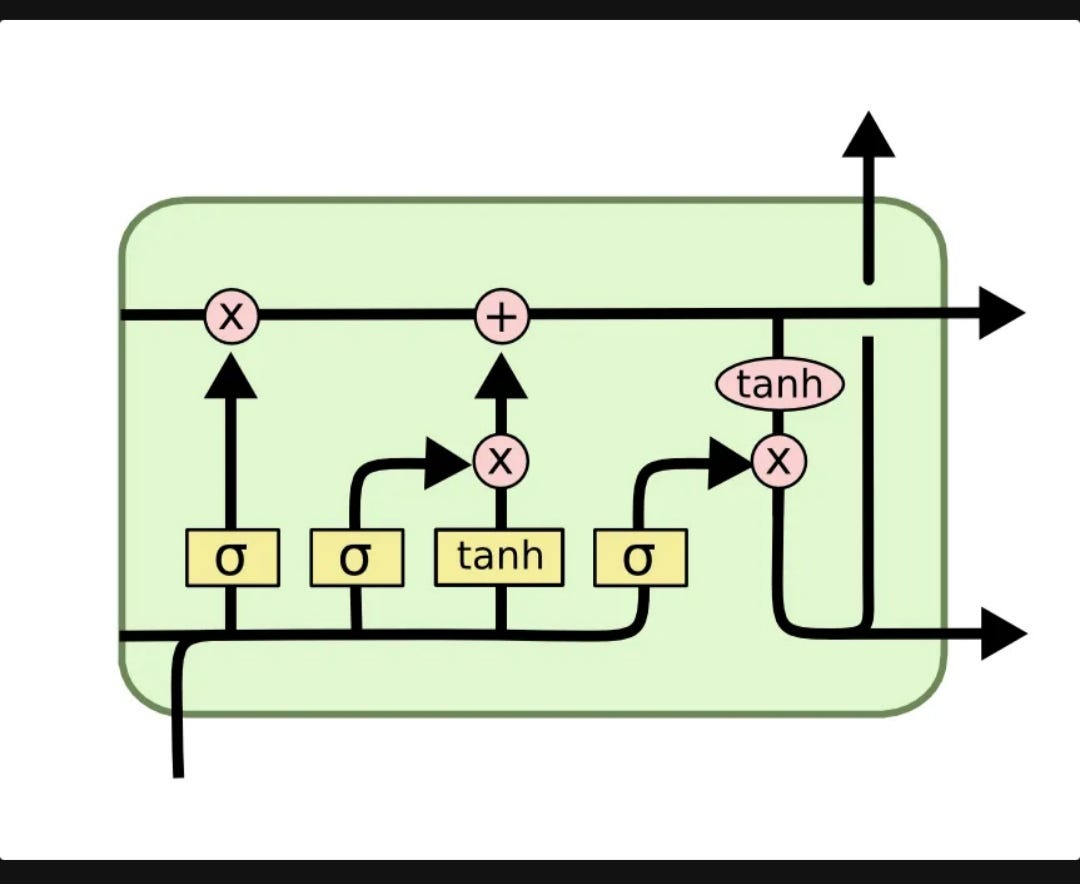
\includegraphics[width=0.45\textwidth,clip,trim=0cm 1.2cm 0cm 1.2cm]{images/lstm.jpg}
    \caption{Esquema representativo de una unidad LSTM con sus compuertas internas.}
    \label{fig:lstm_unit}
\end{figure}


\subsubsection{Convolutional Neural Networks (CNN)}

Las \textbf{Convolutional Neural Networks} (CNN) son un tipo de red neuronal profunda diseñadas originalmente para el procesamiento de datos con estructura espacial, como imágenes o señales. Su principal característica es el uso de capas convolucionales, que aplican filtros locales sobre los datos de entrada para extraer patrones relevantes de forma jerárquica, reduciendo al mismo tiempo el número de parámetros respecto a redes completamente conectadas.

En el contexto de este trabajo, las CNN se emplean en su variante \textit{1D}, donde las convoluciones se aplican sobre el vector de características de cada flujo de red, tratado como una señal unidimensional. Este enfoque permite capturar relaciones locales entre características adyacentes, modelando interacciones de corto alcance entre variables sin necesidad de introducir arquitecturas excesivamente complejas. De este modo, la CNN 1D actúa como una alternativa intermedia entre el MLP y las redes recurrentes, explorando si la extracción local de patrones aporta mejoras en la detección de intrusiones.

Desde el punto de vista computacional, el coste de una CNN depende principalmente del número de filtros, el tamaño del kernel y la profundidad de la red. Aunque las CNN suelen ser más eficientes que otras arquitecturas profundas al compartir pesos, un número elevado de filtros o capas puede incrementar significativamente el tiempo de entrenamiento y la latencia de inferencia. Por esta razón, en este trabajo se utilizan arquitecturas CNN poco profundas y con un número reducido de filtros, priorizando configuraciones compactas y eficientes.

En términos de \textit{Green AI}, la CNN 1D representa un compromiso entre capacidad de representación y eficiencia computacional. Si bien su coste es superior al de modelos clásicos y MLP sencillos, una arquitectura cuidadosamente limitada permite evaluar el impacto de la extracción convolucional de patrones manteniendo un consumo de recursos razonable.

\begin{table}[H]
    \centering
    \caption{Principales hiperparámetros de CNN y su significado.}
    \label{tab:cnn_hyperparams}
    \begin{tabular}{ll}
        \toprule
        \textbf{Hiperparámetro} & \textbf{Significado} \\
        \midrule
        \texttt{filters} & Número de filtros en la capa convolucional \\
        \texttt{kernel\_size} & Tamaño del kernel de convolución (por ejemplo, 3) \\
        \texttt{strides} & Paso de la convolución sobre la entrada \\
        \texttt{padding} & Tipo de relleno aplicado a los bordes (por ejemplo, \textit{same}, \textit{valid}) \\
        \texttt{activation} & Función de activación utilizada en las capas convolucionales (por ejemplo, \textit{relu}) \\
        \texttt{learning\_rate\_init} & Tasa de aprendizaje inicial para el optimizador \\
        \texttt{batch\_size} & Tamaño del lote de muestras para cada actualización de los pesos \\
        \texttt{max\_iter} & Número máximo de iteraciones de entrenamiento \\
        \bottomrule
    \end{tabular}
\end{table}

\begin{figure}[H]
    \centering
    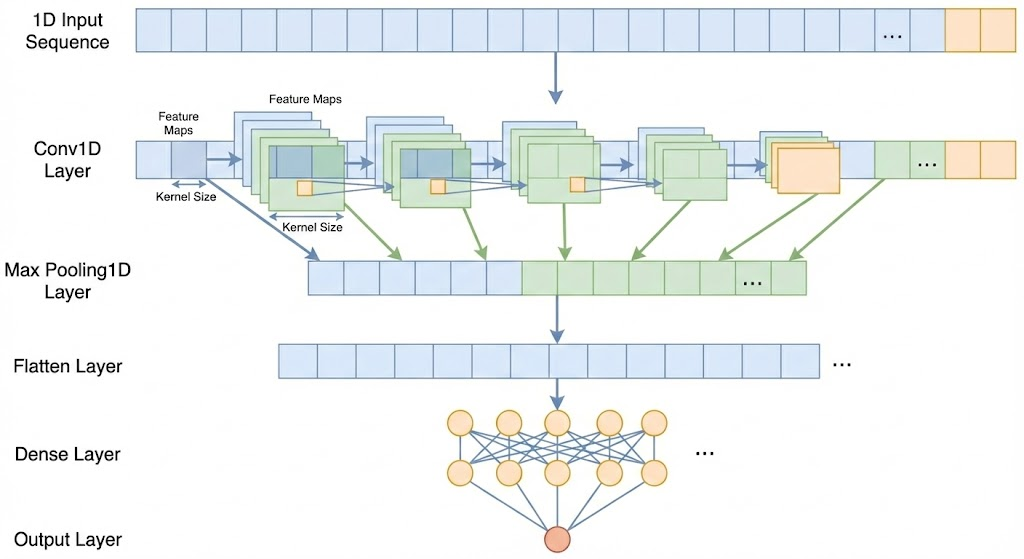
\includegraphics[width=0.7\textwidth]{images/CNN_1D.jpg}
    \caption{Esquema representativo de una arquitectura CNN 1D aplicada a datos tabulares.}
    \label{fig:cnn_1d}
\end{figure}


\section{Optuna}

\textbf{Optuna} es un framework de optimización de hiperparámetros de código abierto que permite a los desarrolladores y científicos de datos encontrar automáticamente los mejores hiperparámetros para sus modelos de aprendizaje automático. Optuna utiliza técnicas de optimización bayesiana para explorar el espacio de hiperparámetros de manera eficiente, lo que puede mejorar significativamente el rendimiento de los modelos.

A diferencia de Grid Search, que realiza una búsqueda exhaustiva y costosa, o Random Search, que no aprende de iteraciones pasadas, Optuna utiliza un enfoque bayesiano basado en el Tree-structured Parzen Estimator (TPE).

El algoritmo TPE construye un modelo probabilístico de la función objetivo. En lugar de probar combinaciones al azar, predice qué regiones del espacio de búsqueda tienen más probabilidades de mejorar los resultados actuales.

Otra de las ventajas de este framework es que nos permite establecer una \textbf{optimización multiobjetivo}, lo que es especialmente útil cuando se desea optimizar varias métricas al mismo tiempo, como la precisión y eficiencia del modelo.

Optuna identifica un conjunto de soluciones que se encuentran en la frontera de Pareto, lo que significa que no hay otra solución que sea mejor en todas las métricas. Esto permite a los usuarios elegir entre diferentes compromisos según sus necesidades específicas, por lo que no presentamos una única solución.

\begin{figure}[H]
    \centering
    \includegraphics[width=0.8\textwidth]{images/OPTUNA.png}
    \caption{Visualización de la optimización con Optuna}
    \label{fig:optuna}
\end{figure}

El procedimiento general aplicado a cada modelo se resume en el Algoritmo~\ref{alg:optuna_cv_multiobjetivo}. Aunque cada arquitectura tiene un espacio de hiperparámetros específico, la estrategia de evaluación se mantiene constante: cada configuración se evalúa mediante validación cruzada estratificada y se optimiza simultáneamente el rendimiento predictivo y el coste de inferencia.

\begin{algorithm}[H]
\caption{Optimización multiobjetivo con validación cruzada estratificada}
\label{alg:optuna_cv_multiobjetivo}
\begin{algorithmic}[1]
\Require Conjunto de entrenamiento completo $D_{train} = (X, y)$, modelo base $M$, espacio de hiperparámetros $\mathcal{H}$, número de ensayos $N$
\Ensure Conjunto de configuraciones evaluadas y frontera de Pareto

\State Crear un estudio de Optuna con dos objetivos:
\Statex \hspace{\algorithmicindent} \textbf{maximizar $F1$ y minimizar la latencia media de inferencia}
\State Definir una validación cruzada estratificada con $K=3$ particiones

\For{cada ensayo $t = 1, \dots, N$}
    \State Seleccionar una configuración de hiperparámetros $h_t \in \mathcal{H}$
    \State Inicializar las listas $F1\_scores$ y $Latencias$

    \For{cada partición $(D_{train}^{(k)}, D_{val}^{(k)})$ de la validación cruzada}
        \State Instanciar el modelo $M_t$ con los hiperparámetros $h_t$
        \State Entrenar $M_t$ sobre $D_{train}^{(k)}$
        \State Obtener las predicciones sobre $D_{val}^{(k)}$
        \State Calcular el $F1$ binario de la clase maliciosa
        \State Añadir el valor obtenido a $F1\_scores$

        \State Seleccionar un subconjunto de validación para medir latencia
        \State Realizar una predicción inicial de calentamiento
        \State Medir varias repeticiones del tiempo de inferencia
        \State Calcular la latencia media por muestra en milisegundos
        \State Añadir la latencia obtenida a $Latencias$
    \EndFor

    \State Calcular $F1_{medio}$ como la media de $F1\_scores$
    \State Calcular $Latencia_{media}$ como la media de $Latencias$
    \State Devolver a Optuna el par $(F1_{medio}, Latencia_{media})$
\EndFor

\State Obtener la frontera de Pareto a partir de todos los ensayos evaluados

\end{algorithmic}
\end{algorithm}

\chapter{Obtención y Análisis de Datos} 
Para cumplir con los objetivos de este Trabajo Fin de Grado, resulta imprescindible realizar una selección cuidadosa de los conjuntos de datos empleados en la fase experimental.

En particular, dado que este trabajo no se centra únicamente en la capacidad de detección, sino también en el rendimiento y el consumo de recursos computacionales, los conjuntos de datos seleccionados deben posibilitar el análisis de aspectos como la latencia de inferencia, el uso de CPU y memoria, y la escalabilidad de los modelos en distintos escenarios. El uso de \textit{datasets} excesivamente simplificados o poco representativos podría conducir a conclusiones poco realistas, mientras que el empleo de conjuntos de datos desproporcionadamente grandes o complejos podría dificultar la reproducibilidad y el análisis experimental detallado.

Por este motivo, en este proyecto se han seleccionado \textit{datasets} ampliamente utilizados en la literatura científica, que cubren diferentes entornos y tipologías de ataque, y que ofrecen un equilibrio adecuado entre realismo, diversidad y viabilidad experimental. Esta elección permite evaluar de forma comparativa el comportamiento de distintos modelos de aprendizaje automático y profundo.

% ======================================================================

\section{UNSW-NB15 \textit{DataSet}}

\subsection{Motivación para el uso del \textit{dataset}}

El conjunto de datos UNSW-NB15 se ha seleccionado como \textit{dataset} principal en este trabajo con el objetivo de proporcionar un escenario más realista y actualizado para la evaluación de sistemas IDS ~\cite{unsw-nb15}. Este \textit{dataset} fue desarrollado por la \emph{University of New South Wales (UNSW)}.

\subsection{Estructura del \textit{dataset}}

El \textit{dataset} UNSW-NB15 está compuesto por registros de tráfico de red generados mediante la combinación de tráfico real y tráfico sintético, con el fin de simular de forma controlada distintos escenarios de ataque en una red corporativa. El conjunto de datos se distribuye en dos archivos principales claramente diferenciados: uno destinado al entrenamiento de los modelos y otro reservado para su evaluación, lo que facilita la reproducibilidad experimental y minimiza el riesgo de \textit{data leakage}.

Cada registro representa un flujo de red y se describe mediante un conjunto de características heterogéneas que incluyen métricas relacionadas con el volumen de tráfico, estadísticas temporales, información de protocolos y atributos derivados del comportamiento de la comunicación. En cuanto a las etiquetas, el \textit{dataset} incorpora una etiqueta binaria que distingue entre tráfico benigno y tráfico malicioso, así como una etiqueta adicional que especifica el tipo de ataque, lo que permite abordar tanto problemas de clasificación binaria como multiclase.


\subsection{Distribución de ataques}


\begin{table}[htbp]
  \centering
  \caption{Distribución de clases y tipos de ataque en el \textit{dataset} UNSW-NB15}
  \label{tab:unsw-nb15-ataques}
  \begin{tabular}{|l|r|}
    \hline
    \textbf{Clase / Tipo de tráfico} & \textbf{Número de flujos} \\
    \hline
    BENIGN & 93\,000 \\
    \hline
    Generic & 58\,871 \\
    Exploits & 44\,525 \\
    Fuzzers & 24\,246 \\
    DoS & 16\,353 \\
    Reconnaissance & 13\,987 \\
    Analysis & 2\,677 \\
    Backdoor & 2\,329 \\
    Shellcode & 1\,511 \\
    Worms & 174 \\
    \hline
    \textbf{Total} & \textbf{257\,673} \\
    \hline
  \end{tabular}
\end{table}

Como puede observarse, aunque el tráfico benigno constituye una parte relevante del \textit{dataset}, una proporción significativa de los registros corresponde a tráfico malicioso, distribuido entre múltiples categorías de ataque. Destacan especialmente las clases \emph{Generic}, \emph{Exploits} y \emph{Fuzzers}, mientras que otras, como \emph{Worms} o \emph{Shellcode}, presentan una frecuencia mucho menor. Esta distribución refleja un escenario realista y resulta adecuada para evaluar el comportamiento de los modelos tanto en términos de detección general de intrusiones como de clasificación específica de ataques.

% ======================================================================

\section{ToN\_IoT \textit{DataSet}}

\subsection{Motivación para el uso del \textit{dataset}}

El conjunto de datos ToN\_IoT (\emph{Telemetry of Network IoT}) se ha incluido en este trabajo con el objetivo de evaluar el comportamiento de los modelos de detección de intrusiones en entornos IoT y \emph{edge computing}, caracterizados por una elevada heterogeneidad, recursos computacionales limitados y requisitos estrictos de eficiencia. Este \textit{dataset} fue desarrollado por la \emph{University of New South Wales (UNSW)} con el propósito de cubrir las limitaciones de los conjuntos de datos tradicionales, que no representan adecuadamente el tráfico ni los patrones de ataque presentes en infraestructuras IoT reales ~\cite{ton-iot}.

\subsection{Estructura del \textit{dataset}}

El \textit{dataset} ToN\_IoT se distribuye en múltiples subconjuntos que incluyen tráfico de red. En concreto, se ha empleado el archivo \texttt{Train\_Test\_Network\_dataset.csv}, que proporciona los datos en formato CSV e incluye una partición predefinida de entrenamiento y prueba. Cada registro representa un flujo de red y se describe mediante un conjunto de características extraídas automáticamente, que abarcan métricas relacionadas con el volumen de tráfico, estadísticas temporales, información de protocolos y atributos derivados del comportamiento de la comunicación.

En cuanto al etiquetado, el \textit{dataset} incorpora una etiqueta binaria que distingue entre tráfico benigno y tráfico malicioso, así como una etiqueta adicional que identifica el tipo de ataque. Esta estructura permite abordar tanto el problema de detección binaria de intrusiones como el análisis de los distintos tipos de tráfico malicioso presentes en entornos IoT.

\subsection{Distribución de ataques}

La distribución de clases del subconjunto de red de ToN\_IoT presenta una proporción equilibrada entre tráfico benigno y varias categorías de ataques, lo que resulta especialmente interesante para evaluar el comportamiento de los modelos en un escenario IoT controlado. En la Tabla~\ref{tab:toniots-ataques} se muestra el número total de flujos correspondiente a cada clase, considerando el conjunto completo de datos.

Como puede observarse, el \textit{dataset} incluye múltiples tipos de ataques representativos de entornos IoT, tales como ataques de denegación de servicio, inyección, escaneo, ransomware y ataques de intermediario (\emph{Man-in-the-Middle}).

\begin{table}[H]
    \centering
    \caption{Distribución de clases y tipos de ataque en el \textit{dataset} ToN\_IoT}
    \label{tab:toniots-ataques}
    \begin{tabular}{|l|r|}
        \hline
        \textbf{Clase / Tipo de tráfico} & \textbf{Número de flujos} \\
        \hline
        BENIGN & 50\,000 \\
        backdoor & 20\,000 \\
        ddos & 20\,000 \\
        dos & 20\,000 \\
        injection & 20\,000 \\
        password & 20\,000 \\
        ransomware & 20\,000 \\
        scanning & 20\,000 \\
        xss & 20\,000 \\
        mitm & 1\,043 \\
        \hline
        \textbf{Total} & \textbf{191\,043} \\
        \hline
    \end{tabular}
\end{table}

% ======================================================================

\section{IoT-23 \textit{Dataset}}

\subsection{Motivación para el uso del \textit{dataset}}

El conjunto de datos \textbf{IoT-23} se ha incorporado en este trabajo como \textit{dataset} complementario orientado a entornos IoT reales. IoT-23, desarrollado por el grupo \emph{Stratosphere IPS} de la \emph{Czech Technical University (CTU)}, es uno de los conjuntos de datos más representativos para el estudio de amenazas dirigidas específicamente a dispositivos IoT ~\cite{iot-23}.

\subsection{Estructura del \textit{dataset}}

IoT-23 se distribuye en forma de escenarios independientes, donde cada escenario corresponde a una captura concreta asociada a un tipo específico de malware o comportamiento malicioso. Estos escenarios se almacenan en directorios separados y presentan tamaños muy variables, desde unos pocos megabytes hasta decenas de gigabytes, lo que dificulta su uso directo en entornos experimentales con recursos limitados.

Con el fin de garantizar la viabilidad experimental y mantener la reproducibilidad de los experimentos, en este trabajo se ha seleccionado un subconjunto reducido de escenarios representativos. En concreto, se han utilizado los archivos \texttt{capture-1-1.labeled} y \texttt{capture-3-1.labeled}, que presentan un tamaño manejable y contienen tráfico IoT real con actividad maliciosa claramente identificable.

\subsection{Distribución de ataques}

La distribución de clases en los escenarios seleccionados de IoT-23 presenta un fuerte desbalanceo entre tráfico benigno y tráfico malicioso, así como una predominancia de determinados comportamientos de ataque característicos de dispositivos IoT comprometidos. En la Tabla~\ref{tab:iot23-ataques} se muestra el número total de flujos correspondiente a cada clase y tipo de tráfico, considerando conjuntamente los archivos \texttt{capture-1-1.labeled} y \texttt{capture-3-1.labeled}.

\begin{table}[H]
    \centering
    \caption{Distribución de clases y tipos de tráfico en el \textit{dataset} IoT-23}
    \label{tab:iot23-ataques}
    \begin{tabular}{|l|r|}
        \hline
        \textbf{Clase / Tipo de tráfico} & \textbf{Número de flujos} \\
        \hline
        Malicious -- PartOfAHorizontalPortScan & 685\,062 \\
        Benign & 473\,811 \\
        Malicious Attack & 5\,962 \\
        Malicious -- C\&C & 16 \\
        \hline
        \textbf{Total} & \textbf{1\,164\,851} \\
        \hline
    \end{tabular}
\end{table}

Como puede observarse, el tráfico malicioso asociado a escaneos horizontales de puertos domina el conjunto de datos.

\section{Relación entre los \textit{datasets}}

Los tres \textit{datasets} proporcionan características extraídas a nivel de flujo de red (estadísticas de paquetes, bytes, duraciones, banderas TCP) a partir de capturas reales.
Todos ellos reflejan la realidad de las redes actuales, donde el tráfico normal (benigno) suele ser la clase mayoritaria. Debido a este desbalanceo, usamos como métrica principal comparativa el F1-score.
Todos los \textit{datasets} son \textit{datasets} reconocidos en la literatura de los análisis de IDS, ya que están diseñados específicamente para el entrenamiento y auditoría de algoritmos de Machine Learning y Deep Learning.

No obstante, también se han elegido porque presentan algunas diferencias entre ellos y así poder ver los resultados de \textit{datasets} que tienen distinta distribución y topología. 
Por ejemplo, UNSW-NB15 está enfocado en una red corporativa tradicional y sirve como punto de referencia base para comprobar que nuestros modelos sepan cazar amenazas usuales.

Por otro lado, los \textit{datasets} IoT-23 y ToN-IoT están enfocados en entornos puramente de IoT donde las capturas provienen de amenazas de infecciones reales de malware en dispositivos inteligentes.

A continuación se muestra una tabla simplificada que resume las características principales de UNSW-NB15:

\begin{table}[H]
\centering
\caption{Correspondencia principal entre características de UNSW-NB15}
\label{tab:relacion-cic-unsw}
\begin{tabular}{|l|l|}
\hline
\textbf{Categoría} & \textbf{UNSW-NB15} \\
\hline
Duración flujo & dur \\
Intervalo paquetes origen & sinpkt \\
Intervalo paquetes destino & dinpkt \\
Paquetes origen & spkts \\
Paquetes destino & dpkts \\
Bytes origen & sbytes \\
Bytes destino & dbytes \\
Tasa paquetes & rate \\
Tamaño medio paquetes origen & smean \\
Tamaño medio paquetes destino & dmean \\
SYN flag & synack \\
ACK flag & ackdat \\
Etiqueta & label / attack\_cat \\ 
\hline
\end{tabular}
\end{table}

Ahora relacionamos los \textit{datasets} ToN\_IoT y IoT-23, destacando las características comunes.
\begin{table}[H]
\centering
\caption{Correspondencia principal entre características de ToN\_IoT e IoT-23}
\label{tab:correspondencia-toniot-iot23}
\begin{tabularx}{\textwidth}{|l|l|l|X|}
\hline
\textbf{Categoría} & \textbf{ToN\_IoT} & \textbf{IoT-23} & \textbf{Descripción} \\
\hline
IP origen & src\_ip & id.orig\_h & Dirección IP origen \\
Puerto origen & src\_port & id.orig\_p & Puerto origen \\
IP destino & dst\_ip & id.resp\_h & Dirección IP destino \\
Puerto destino & dst\_port & id.resp\_p & Puerto destino \\
Protocolo & proto & proto & Protocolo de transporte \\
Duración & duration & duration & Duración de la conexión \\
Bytes origen & src\_bytes & orig\_bytes & Bytes enviados por el origen \\
Bytes destino & dst\_bytes & resp\_bytes & Bytes enviados por el destino \\
Paquetes origen & src\_pkts & orig\_pkts & Paquetes enviados por el origen \\
Paquetes destino & dst\_pkts & resp\_pkts & Paquetes enviados por el destino \\
Estado & conn\_state & conn\_state & Estado de la conexión \\
Etiqueta & label & label & Tráfico benigno o malicioso \\
Tipo ataque & type & detailed-label & Tipo de ataque \\
\hline
\end{tabularx}
\end{table}

\subsection{Justificación del enfoque en la fase de inferencia}

En el contexto de los Sistemas de Detección de Intrusiones (IDS) basados en inteligencia artificial, resulta fundamental distinguir entre la fase de entrenamiento del modelo y la fase de inferencia. Aunque el entrenamiento puede implicar un coste computacional elevado, este proceso se realiza de manera puntual o con una frecuencia reducida. Por el contrario, la fase de inferencia se ejecuta de forma continua una vez que el modelo está desplegado en un entorno real, analizando de manera permanente el tráfico de red entrante.

El coste asociado a la inferencia es el que determina la viabilidad práctica del sistema. Un modelo con excelente rendimiento predictivo pero con alta latencia o consumo excesivo de CPU y memoria puede resultar inviable para su despliegue en tiempo real. Por este motivo, el presente trabajo centra su análisis experimental en el consumo computacional durante la fase de inferencia.

Desde la perspectiva de la Green AI, esta decisión está alineada con el objetivo de reducir el consumo energético en sistemas de uso continuo. Mientras que el entrenamiento representa un coste energético puntual, la inferencia constituye un coste acumulativo y sostenido en el tiempo. Por tanto, optimizar la eficiencia en esta fase tiene un impacto directo en la sostenibilidad del sistema IDS.

\subsection{Optimización de hiperparámetros estructurales}

Dado que el objetivo principal es analizar el equilibrio entre capacidad de detección y eficiencia computacional en inferencia, el ajuste de hiperparámetros se centra específicamente en aquellos que determinan la estructura del modelo. Los hiperparámetros estructurales influyen directamente en la complejidad computacional, el número de operaciones necesarias para generar una predicción y el tamaño final del modelo.

A diferencia de otros hiperparámetros relacionados con el proceso de entrenamiento (como la tasa de aprendizaje o el optimizador), los hiperparámetros estructurales determinan la arquitectura final del modelo y, por tanto, su coste en tiempo de ejecución una vez desplegado.

A continuación, se describen los hiperparámetros estructurales más relevantes para cada uno de los modelos considerados en este trabajo.

\subsubsection{Random Forest}

En el caso de Random Forest, el coste de inferencia depende principalmente de:

\begin{itemize}
    \item \textbf{n\_estimators}: número de árboles que componen el bosque. Un mayor número de árboles incrementa linealmente el número de recorridos necesarios para cada predicción.
    \item \textbf{max\_depth}: profundidad máxima de cada árbol. Árboles más profundos implican más comparaciones por predicción.
\end{itemize}

\subsection{XGBoost}

En XGBoost, la inferencia consiste en recorrer secuencialmente todos los árboles entrenados y sumar sus contribuciones. Los hiperparámetros estructurales más relevantes son:

\begin{itemize}
    \item \textbf{n\_estimators}: número total de árboles del modelo.
    \item \textbf{max\_depth}: profundidad máxima de cada árbol.
\end{itemize}

\subsection{Support Vector Machine (SVM)}

Para SVM, el coste de inferencia depende principalmente del tipo de kernel utilizado. En este trabajo se prioriza el uso de:

\begin{itemize}
    \item \textbf{kernel lineal}: permite realizar predicciones mediante un producto escalar, lo que reduce significativamente el coste computacional.
    \item \textbf{C}: parámetro de regularización que puede influir en la complejidad del modelo, aunque su impacto en la inferencia es menor que el tipo de kernel.
\end{itemize}

\subsection{Multilayer Perceptron (MLP)}

En redes MLP, el coste de inferencia está directamente relacionado con el número total de pesos del modelo. Los hiperparámetros estructurales clave son:

\begin{itemize}
    \item \textbf{hidden\_layer\_sizes}: número de capas ocultas y número de neuronas por capa.
\end{itemize}

\subsection{Long Short-Term Memory (LSTM)}

En las redes LSTM, la complejidad de inferencia depende de:

\begin{itemize}
    \item \textbf{units}: número de unidades LSTM en la capa recurrente.
    \item \textbf{longitud de secuencia}: número de pasos temporales procesados.
\end{itemize}


\subsection{Convolutional Neural Networks (CNN 1D)}

En las CNN 1D utilizadas en este trabajo, los hiperparámetros estructurales más relevantes son:

\begin{itemize}
    \item \textbf{filters}: número de filtros en las capas convolucionales.
    \item \textbf{kernel\_size}: tamaño del kernel.
    \item \textbf{número de capas convolucionales}.
    \item \textbf{Stride}: si aumentas el stride, reduces el número de operaciones de convolución, lo cual acelera drásticamente la inferencia.
\end{itemize}


\section{Resultados}

\subsection{Random Forest}

Para el modelo de Random Forest, utilizando Optuna, se han obtenido los siguientes resultados como frontera de Pareto:
\begin{figure}[h]
    \centering
    
\includegraphics[width=0.8\textwidth]{../../images/PARETO_RF.png}
    \caption{Frontera de Pareto - Random Forest}
    \label{fig:pareto_rf}
\end{figure}

Se observa que configuraciones con un número reducido de árboles (n=50) y elevada profundidad (max_depth≈29) alcanzan valores de F1-macro prácticamente equivalentes a los modelos de mayor tamaño, pero con una latencia aproximadamente seis veces inferior. Este resultado evidencia que el incremento del número de árboles produce rendimientos decrecientes en términos de eficacia, mientras que el coste computacional continúa aumentando de forma significativa.

Hemos visto cómo reaccionan en test los modelos con los siguientes hiperparámetros elegidos:

1. (50, 29) Con solo 50 árboles alcanza un F1 casi idéntico al de modelos mucho más pesados
2. (100, 25) Es un punto intermedio, duplica los árboles respecto al anterior, pero gana robustez
3. (300, 28) Es más lento que los 3, pero es el que más F1 tiene

Los resultados son los siguientes:

\begin{table}[h]
    \centering
    \begin{tabular}{|l|c|c|c|c|c|}
        \hline
        \textbf{Perfil} & \textbf{n\_estimators} & \textbf{max\_depth} & \textbf{F1\_Test} & \textbf{Accuracy\_Test} & \textbf{Latencia (ms)} \\
        \hline
        Alta Eficiencia & 50 & 29 & 0.8731 & 0.8774 & 0.0012 \\
        \hline
        Equilibrado & 100 & 25 & 0.8809 & 0.8845 & 0.0018 \\
        \hline
        Máxima Precisión & 300 & 28 & 0.8766 & 0.8807 & 0.0055 \\
        \hline
    \end{tabular}
    \caption{Comparativa final de modelos Random Forest en el set de test}
    \label{tab:rf_comparison}
\end{table}
\section{Evaluación de robustez frente a ataques adversarios}

Hasta este punto del trabajo, los modelos de detección de intrusiones desarrollados han mostrado un rendimiento muy elevado sobre los conjuntos de prueba originales. En particular, las arquitecturas profundas, como MLP y CNN-1D, han alcanzado valores de F1-score superiores al 96\%, mientras que los modelos basados en ensambles de árboles de decisión, como Random Forest, XGBoost, LightGBM y CatBoost, han obtenido resultados cercanos al 99\%. Estos resultados indican que los modelos son capaces de aprender patrones relevantes en los datasets empleados y ofrecen una alta capacidad de clasificación en condiciones normales de evaluación.

Sin embargo, en el ámbito de la ciberseguridad, un buen rendimiento sobre datos estáticos no garantiza por sí solo que un sistema sea robusto en escenarios reales. Los atacantes pueden conocer o inferir el funcionamiento de los sistemas de detección y adaptar su comportamiento para evadirlos. En este contexto surge el aprendizaje automático adversario, cuyo objetivo es estudiar cómo pequeñas modificaciones en las entradas pueden provocar errores de clasificación en modelos de inteligencia artificial.

En el caso de los sistemas de detección de intrusiones en red, los ataques de evasión se producen durante la fase de inferencia. En este tipo de ataques, una muestra maliciosa se modifica de forma controlada para intentar que el modelo la clasifique como tráfico benigno. Por ejemplo, un flujo asociado a un ataque de denegación de servicio, un escaneo de puertos o una comunicación maliciosa podría ser alterado ligeramente con el objetivo de desplazarlo al lado benigno de la frontera de decisión del clasificador. Si el ataque tiene éxito, el sistema dejaría de generar una alerta, reduciendo así su utilidad en un entorno operativo.

Para analizar esta problemática, en esta fase del proyecto se evaluará la robustez adversaria de los modelos finales seleccionados en las etapas anteriores. Es importante destacar que no se realizará una nueva optimización de hiperparámetros, sino que se partirá de las configuraciones ya elegidas para cada modelo. De este modo, la evaluación adversaria se plantea como una prueba adicional de resistencia sobre los modelos previamente considerados como mejores bajo condiciones limpias.

\subsection{Uso de Adversarial Robustness Toolbox}

La herramienta principal empleada para esta evaluación será \textit{Adversarial Robustness Toolbox} (ART), una librería orientada al análisis de seguridad y robustez de modelos de aprendizaje automático. ART proporciona implementaciones estandarizadas de ataques adversarios utilizados habitualmente en la literatura, como FGSM, BIM o PGD, y permite integrarlos con modelos desarrollados en distintos entornos de aprendizaje automático y aprendizaje profundo.

La elección de ART frente a otras alternativas, como CleverHans o Torchattacks, se debe principalmente a su carácter generalista y a su integración con distintos tipos de modelos. En el contexto de este trabajo, esta característica resulta especialmente útil, ya que el conjunto de modelos evaluados es heterogéneo e incluye tanto arquitecturas neuronales como clasificadores clásicos y métodos de ensamble.

La evaluación de robustez de los distintos clasificadores NIDS propuestos en este trabajo exige adaptar la estrategia de ataque a la naturaleza matemática subyacente de cada algoritmo. Por este motivo, se ha diseñado una metodología en dos fases, basada en ataques directos y en la transferencia de vulnerabilidades.

\subsubsection{1. Ataques de Caja Blanca basados en Gradiente (MLP y CNN-1D)}

Los algoritmos de evasión empleados en este estudio, como \textit{Projected Gradient Descent} (PGD) o \textit{Fast Gradient Sign Method} (FGSM), requieren de un requisito matemático indispensable: \textbf{el modelo objetivo debe ser continuo y diferenciable}. 

En arquitecturas de aprendizaje profundo como el Perceptrón Multicapa (MLP) y las Redes Neuronales Convolucionales (CNN-1D), el atacante emplea la retropropagación (\textit{backpropagation}) para calcular el gradiente de la función de pérdida con respecto a las características de entrada. Esto permite identificar la dirección matemática exacta para alterar el tráfico de red original e inducir a una clasificación errónea (falsos negativos). Además, durante este proceso iterativo, se aplican estrictas restricciones de dominio (\textit{Domain Constraints}) para garantizar que las características categóricas y los límites físicos de los protocolos de red se mantengan inalterados, preservando la viabilidad del ataque en un entorno real.

\subsubsection{2. Transferencia Adversaria para Modelos Discretos (Ensambles y SVM)}

A diferencia de las redes neuronales, los modelos que fundamentan sus decisiones en particiones del espacio paramétrico, como los ensambles de árboles de decisión (Random Forest, XGBoost, LightGBM, CatBoost) o las Máquinas de Vectores de Soporte (SVM), presentan fronteras lógicas abruptas que inutilizan la aplicación directa del cálculo de gradientes.

Para solventar esta limitación e incorporar estos algoritmos a la evaluación de seguridad, se explota la técnica de \textbf{Transferencia Adversaria} (\textit{Adversarial Transferability}). Esta estrategia asume que las perturbaciones diseñadas para engañar a un modelo específico suelen evadir con éxito clasificadores con arquitecturas completamente distintas. El procedimiento aplicado es el siguiente:

\begin{enumerate}
    \item \textbf{Generación (\textit{White-box}):} Los modelos diferenciables (MLP y CNN-1D) actúan como modelos sustitutos (\textit{surrogate models}) para la generación algorítmica del nuevo conjunto de tráfico de red evadido, denominado \textit{Dataset Adversario}.
    \item \textbf{Evaluación Cruzada (\textit{Black-box}):} El \textit{Dataset Adversario} se introduce directamente en la fase de inferencia de los clasificadores basados en árboles y SVM.
    \item \textbf{Cuantificación del Impacto:} Se mide la degradación de las métricas de rendimiento frente al estado basal.
\end{enumerate}

%────────────────────── Contraportada ──────────────────────────────────
\backmatter
\nocite{*}
\printbibliography[heading=bibintoc,title={Bibliografía}]
\cleardoublepage
\MakeUMABackCover
\end{document}
% ======================================================================
